\section{Evaluation}
We have implemented a demo version of our benchmark.
It now can work on a single node,
and measure classic network metrics such as throughput and latency.
In this section, we evaluate the first two chains in Table \ref{chains}. 
The testbed we used for our evaluation builds on an general server (Intel Xeon E5V3-2658 2.2GHz, 12 cores, 32GB, 2$\times$1Gbps NICs) which runs CentOS 7 system, with Kubernetes 1.4 and Open vSwitch 2.5.1. We encapsulates NFs with Docker 1.12.5 running Ubuntu 14.14. 

%\subsection{Throughput}

%\begin{figure}[t]
%\label{cdf}
%\centering
%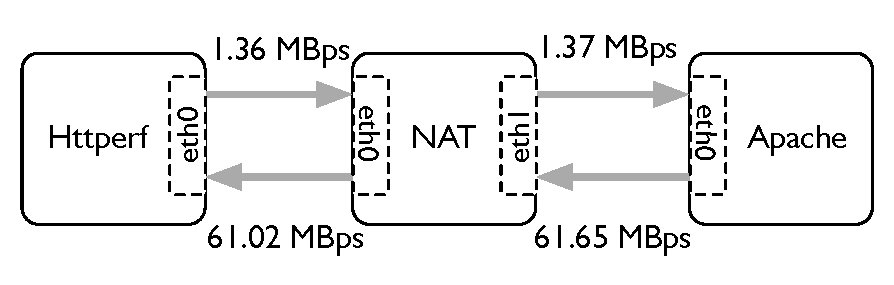
\includegraphics[width=3.3in]{throughput_chain1.eps}
%\caption{Throughput of each NF of SFC1.}
%\end{figure}
%
%\begin{figure}[t]
%\label{cdf}
%\centering
%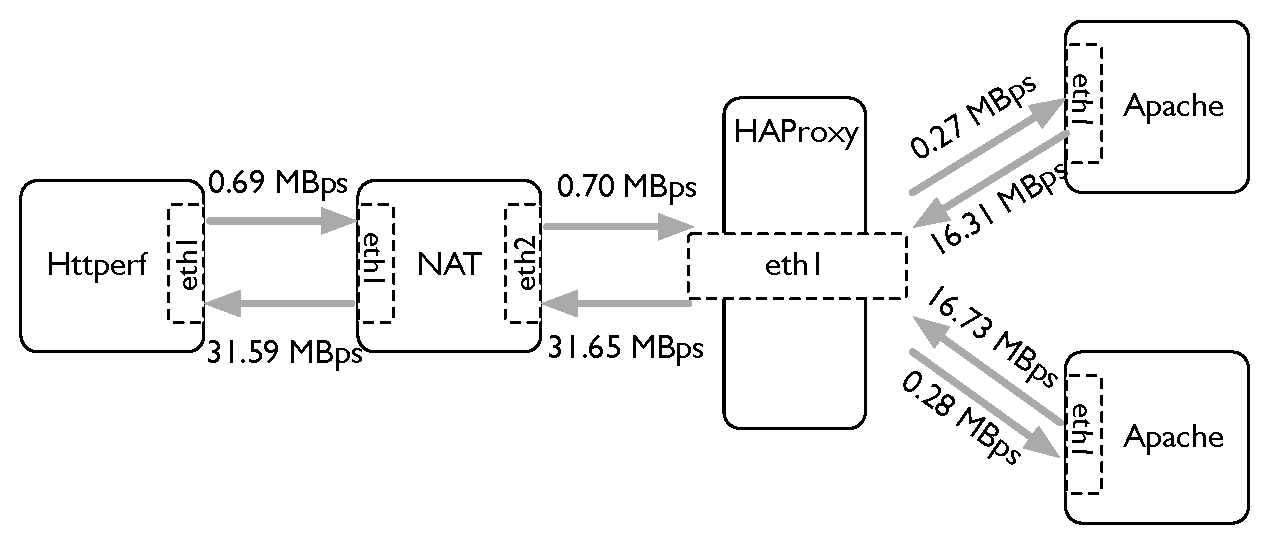
\includegraphics[width=3.3in]{throughput_chain2.eps}
%\caption{Throughput of each NF of SFC2.}
%\end{figure}

\begin{figure}[!t]
\centering
\subfloat[SFC1]{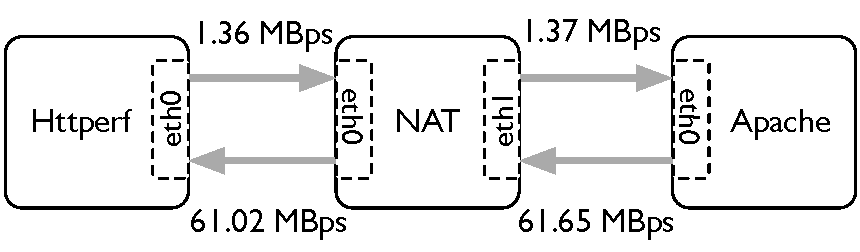
\includegraphics[width=3.3in]{fig/throughput_chain1.pdf}
\label{throughput_SFC1}}
\hfil
\subfloat[SFC2]{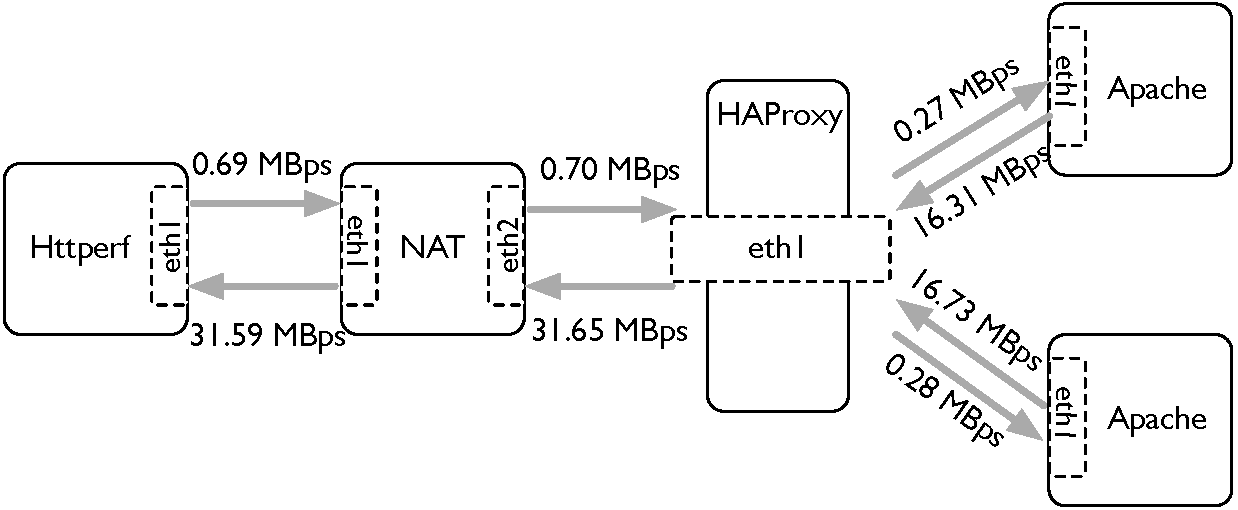
\includegraphics[width=3.3in]{fig/throughput_chain2.pdf}
\label{throughput_SFC2}}
\hfil
\caption{Throughput of each NF}
\label{throughput}
\end{figure}


\begin{figure}[t]
\centering
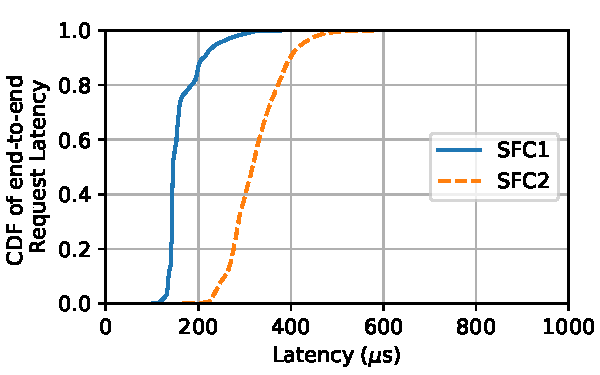
\includegraphics[width=3.3in]{fig/e2e_latency_chain12.pdf}
\caption{End-to-end request latency of SFC1 and SFC2.}
\label{e2e_latency}
\end{figure}

We measure throughput of each container using Docker API. 
The transmit bytes and receive bytes are recorded two times 
at the begin and end of test running respectively. 
Throughput of each NF is calculated 
by doing subtraction of transmit bytes and divid it by the testing time. 
We also measured end-to-end request latency by modifying the workload generator Httperf. 
It records the latency of each request and output the distribution of latencies.

Figure \ref{throughput} shows the topology of two chains 
and the throughput are labeled on the arrows. 
The direction of the arrows indicates the flow of the packets.



%\subsection{Latency}


\begin{figure}[t]
\centering
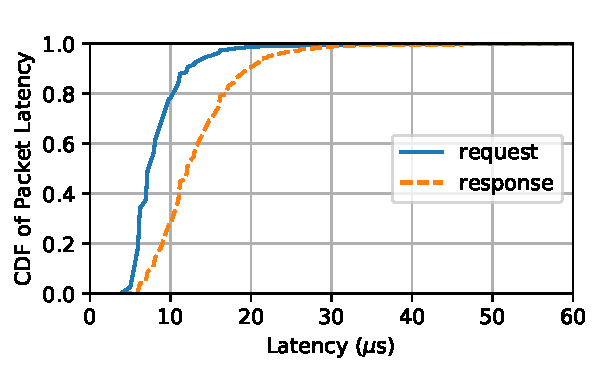
\includegraphics[width=3.3in]{fig/cdf_chain1.pdf}
\caption{Per-packet latency of NAT in SFC1}
\label{nat_latency}
\end{figure}

Figure \ref{e2e_latency} shows the end to end latency of SFC1 and SFC2. 
Figure \ref{nat_latency} shows the per-packet latency of NAT in SFC1. 




